\documentclass[a4paper,12pt]{article}
\usepackage{amsmath}
\usepackage{tikz}
\usetikzlibrary{automata, positioning, arrows.meta}
\usepackage{fontspec}
\usepackage{float}     % Для [H]
\setmainfont{Times New Roman}
\usepackage[russian]{babel}
\usepackage{graphicx}
\usepackage{geometry}
\geometry{left=3cm,right=1.5cm,top=2cm,bottom=2cm}
\usepackage{setspace}
\onehalfspacing
\linespread{1.5}
\setlength{\parindent}{1.25cm}

\title{%
  \begin{center}
    
\includegraphics{../assets/gerb.png}
  \end{center}
  {\large МИНИСТЕРСТВО НАУКИ И ВЫСШЕГО ОБРАЗОВАНИЯ РОССИЙСКОЙ
  ФЕДЕРАЦИИ}\\
  {\normalsize Федеральное государственное бюджетное образовательное
  учреждение высшего образования}\\
  {\large \textbf{«МИРЭА --- Российский технологический университет»}}\\
  {\normalsize РТУ МИРЭА}\\
  {\normalsize Институт искусственного интеллекта (ИИИ)}\\
  {\normalsize Кафедра Промышленной информатики (ПИ)}\\
  {\LARGE \textbf{ОТЧЕТ}}\\
  {\Large \textbf{ПО ПРАКТИЧЕСКОЙ РАБОТЕ № 11}}\\
  {\large \textbf{по дисциплине «Информатика»}}
}
\author{%
  \begin{tabular}{ll}
    Выполнил студент группы КВБО-11-25 & Шапаренко Ф.А. \\
    Принял ассистент        & Беднов Г.А. \\
  \end{tabular}
}
\date{%
  Практическую работу выполнил «16» 03 2026 г.\\
  «Зачтено» «»  2026 г.\\
  Москва 2026
}

\begin{document}
\maketitle

\noindent\textbf{Тема:} «Исследование триггеров»\\
\noindent\textbf{Цель работы:} \\
- изучение структуры и алгоритмов
работы асинхронных и
синхронных триггеров; \\
- исследование функций переходов и возбуждения основных
типов триггеров; \\
- изучение взаимозаменяемости триггеров различных типов.

\begin{figure}[h]
  \centering
  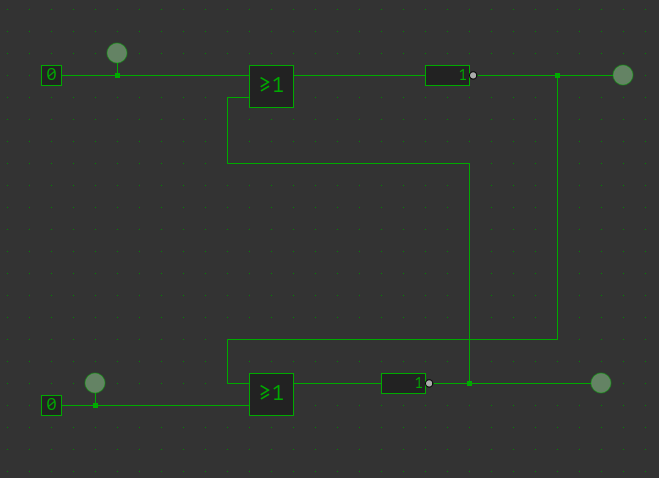
\includegraphics[width=0.8\textwidth]{../assets/scheme.png}
  \caption{схема работы RS тригера}
\end{figure}

\begin{center}
  \begin{tabular}{|c|c|c|}
    \hline
    S & R & \(Q_{n+1}\) \\ \hline
    0 & 0 & \(Q_n\) \\ \hline
    0 & 1 & 0 \\ \hline
    1 & 0 & 1 \\ \hline
    1 & 1 & --- \\ \hline
  \end{tabular}
\end{center}

\begin{center}
  \begin{tabular}{|c|c|c|c|}
    \hline
    \(Q_n\) & \(Q_{n+1}\) & S & R \\ \hline
    0 & 0 & 0 & x \\ \hline
    0 & 1 & 1 & 0 \\ \hline
    1 & 0 & 0 & 1 \\ \hline
    1 & 1 & x & 0 \\ \hline
  \end{tabular}
\end{center}

\begin{figure}[H]
  \centering
  \begin{tikzpicture}[> = stealth, auto, thick]
    \node[state] (0) {0};
    \node[state] (1) [right=4cm of 0] {1};

    \path[->] (0) edge [loop left] node[below=0.1cm] {\(S = 0\)} ()
    (1) edge [loop right] node [above=0.1cm] {\(R=0\)} ()
    (0) edge [bend right] node [below] {\(SR=10\)} (1)
    (1) edge [bend right] node [above] {\(SR=01\)} (0);
  \end{tikzpicture}
  \caption{Схема работы SR триггера}
\end{figure}

\begin{figure}[h]
  \centering
  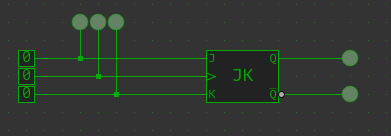
\includegraphics[width=0.8\textwidth]{../assets/JK.png}
  \caption{JK триггер}
\end{figure}

\begin{center}
  \begin{tabular}{|c|c|c|c|c|l|}
    \hline
    C & J & K & \(Q_n\) & \(Q_{n+1}\) & \text{Режим работы} \\
    \hline
    0 & \(x\) & \(x\) & 0 & 0 & \text{Хранение} \\
    0 & \(x\) & \(x\) & 1 & 1 & \text{Хранение} \\
    \hline
    1 & 0 & 0 & 0 & 0 & \text{Хранение} \\
    1 & 0 & 0 & 1 & 1 & \text{Хранение} \\
    \hline
    1 & 0 & 1 & \(x\) & 0 & \text{Сброс} \\
    \hline
    1 & 1 & 0 & \(x\) & 1 & \text{Установка} \\
    \hline
    1 & 1 & 1 & 0 & 1 & \text{Инверсия} \\
    1 & 1 & 1 & 1 & 0 & \text{Инверсия} \\
    \hline
  \end{tabular}
\end{center}

\begin{center}
  \begin{tabular}{|c|c|c|c|l|}
    \hline
    \(Q_n\) & \(Q_{n+1}\) & J & K & \text{Режим работы} \\
    \hline
    0 & 0 & 0 & \(x\) & Хранение 0 или Сброс \\
    \hline
    0 & 1 & 1 & \(x\) & Установка 1 или Инверсия \\
    \hline
    1 & 0 & \(x\) & 1 & Сброс 0 или Инверсия \\
    \hline
    1 & 1 & \(x\) & 0 & Хранение 1 или Установка \\
    \hline
  \end{tabular}
\end{center}

\begin{figure}[H]
  \centering
  \begin{tikzpicture}[> = stealth, auto, thick]
    \node[state] (0) {0};
    \node[state] (1) [right=4cm of 0] {1};

    \path[->] (0) edge [loop left] node[below=0.1cm] {\(J = 0\)} ()
    (1) edge [loop right] node [above=0.1cm] {\(K=0\)} ()
    (0) edge [bend right] node [below] {\(J=1\)} (1)
    (1) edge [bend right] node [above] {\(K=1\)} (0);
  \end{tikzpicture}
  \caption{Схема работы JK триггера}
\end{figure}

\begin{figure}[h]
  \centering
  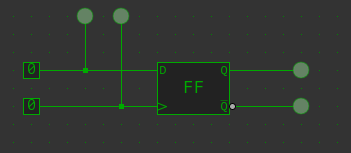
\includegraphics[width=0.8\textwidth]{../assets/D триггер.png}
  \caption{D триггер}
\end{figure}

\begin{center}
  \begin{tabular}{|c|c|c|c|c|}
    \hline
    C & D & $Q_{n}$ & $Q_{n+1}$ & Режим \\
    \hline
    0 & $x$ & $Q_{n}$ & $Q_{n}$ & Хранение \\
    \hline
    1 & 1 & $x$ & 1 & Запись 1 \\
    \hline
    1 & 0 & $x$ & 0 & Запись 0 \\
    \hline
  \end{tabular}
\end{center}

\begin{center}
  \begin{tabular}{|c|c|c|c|}
    \hline
    $Q_n$ & $Q_{n+1}$ & D & Режим \\
    \hline
    0 & 0 & 0 & Сохранение состояния 0 \\
    \hline
    0 & 1 & 1 & Переход в состояние 1 \\
    \hline
    1 & 0 & 0 & Переход в состояние 0 \\
    \hline
    1 & 1 & 1 & Сохранение состояния 1 \\
    \hline
  \end{tabular}
\end{center}

\begin{figure}[H]
  \centering
  \begin{tikzpicture}[> = stealth, auto, thick]
    \node[state] (0) {0};
    \node[state] (1) [right=4cm of 0] {1};

    \path[->] (0) edge [loop left] node[below=0.1cm] {\(D = 0\)} ()
    (1) edge [loop right] node [above=0.1cm] {\(D=0\)} ()
    (0) edge [bend right] node [below] {\(D=1\)} (1)
    (1) edge [bend right] node [above] {\(D=0\)} (0);
  \end{tikzpicture}
  \caption{Схема работы D триггера}
\end{figure}

\end{document}
